\documentclass[xcolor=dvipsnames]{beamer}
%==============================================================================
% PACOTES UTILIZADOS
%------------------------------------------------------------------------------
% Contém as configurações visuais da apresentação e carrega alguns pacotes
% utilizados na apresentação
\usepackage{OliveGreenStyle}
%------------------------------------------------------------------------------
% Pacotes de linguagem e codificação
\usepackage[T1]{fontenc} 
\usepackage{ae} 
\usepackage[utf8]{inputenc}
\usepackage[brazil]{varioref}
\usepackage[brazil,brazilian,english]{babel}
%------------------------------------------------------------------------------
%==============================================================================
% INFORMAÇÕES PARA A PÁGINA DE TÍTULOS
%------------------------------------------------------------------------------
\title{Aplicação de métodos estatísticos para comparação de modelos de otimização}
%------------------------------------------------------------------------------
%------------------------------------------------------------------------------
\author
{
	Gustavo Marques Zeferino \\
}
\institute{SACSIS 2013}
%------------------------------------------------------------------------------
\date{22 de novembro de 2013}
%------------------------------------------------------------------------------

%******************************************************************************
% INICIO DO DOCUMENTO
%******************************************************************************
\begin{document}
%******************************************************************************

%==============================================================================

\frame{\titlepage} %página de rosto

%==============================================================================

% cria o sumario
%\begin{frame}%-----------------------------------------------------------------
	%\frametitle{Sumário}
	%\tableofcontents
	%Cada seção é um slide
	%\tableofcontents[pausesections]

%\end{frame}%-------------------------------------------------------------------

%==============================================================================

\section{Otimização}

\subsection{Introdução}

\begin{frame}%-----------------------------------------------------------------
\frametitle{Otimização}

\begin{block}{Conceito}
Em matemática, o termo otimização, ou programação matemática, refere-se ao estudo de problemas em que se busca minimizar ou maximizar uma função através da escolha sistemática dos valores de variáveis reais ou inteiras dentro de um conjunto viável.
\end{block}

\end{frame}%-------------------------------------------------------------------

\begin{frame}%-----------------------------------------------------------------
\frametitle{Tipos de problemas de otimização}

\begin{itemize}
\item Otimização contínua
\[
\begin{array}{lll}
 \displaystyle\min_{x}          & f(x) & \\
 \mbox{sujeito a} & g(x)_{i} \leq 0, &  i = 1, \ldots, m \\
                  & h(x)_{i} = 0, &  i = 1, \ldots, p \\
\end{array}
\]
onde
\begin{itemize}
\item $f(x): \mathbb{R}^{n} \rightarrow \mathbb{R}$ é a função objetivo
\item $g(x)_{i} \leq 0 $ são restrições de desigualdade
\item $h(x)_{i} = 0 $ são restrições de igualdade
\end{itemize}



\end{itemize}

\end{frame}%-------------------------------------------------------------------


\begin{frame}%-----------------------------------------------------------------
\frametitle{Tipos de problemas de otimização}

\begin{itemize}
\item Otimização discreta ou combinatória é quádruplo (I, f, m, G), onde

\begin{itemize}
\vspace{10pt}\item $I$ é um conjunto de instâncias
\vspace{10pt}\item Dada uma instância, $x \in I$, $f(x)$ é um conjunto de soluções viáveis
\vspace{10pt}\item Dada uma instância $x$ e uma solução viável $y$ de $x$, $m(x,y)$ denota a medida de $y$, que é usualmente um número real positivo
\vspace{10pt}\item $G$ é a função objetivo, e é tanto mínimo ou máximo.
\end{itemize}

\end{itemize}

\end{frame}%-------------------------------------------------------------------



\subsection{Exemplos}

\begin{frame}%-----------------------------------------------------------------
\frametitle{Otimização de uma função contínua}
\begin{figure}
\centering
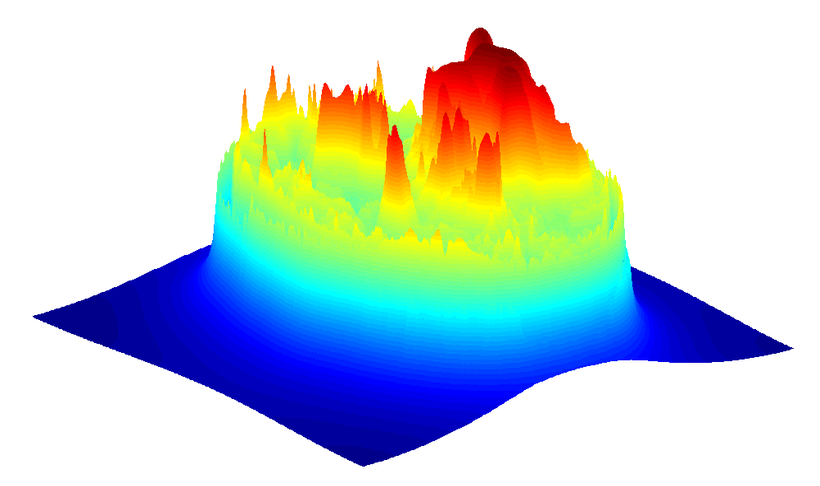
\includegraphics[scale=0.4]{img/opt_function.png}
\end{figure}
\end{frame}%-------------------------------------------------------------------


\begin{frame}%-----------------------------------------------------------------
\frametitle{Problema do caixeiro viajante}
\begin{figure}
\centering
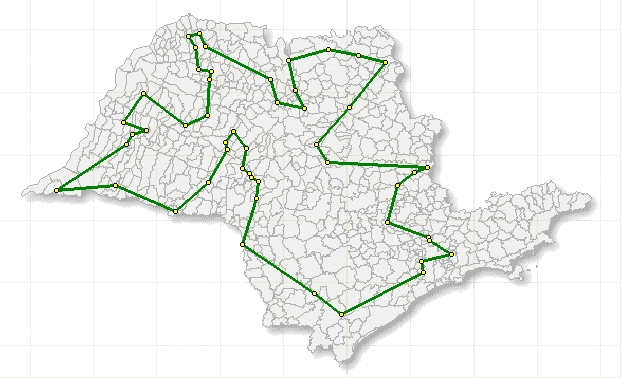
\includegraphics[scale=0.5]{img/tsp.jpg}
\end{figure}
\end{frame}%-------------------------------------------------------------------

\begin{frame}%-----------------------------------------------------------------
\frametitle{Problema de corte e empacotamento}
\begin{figure}
\centering
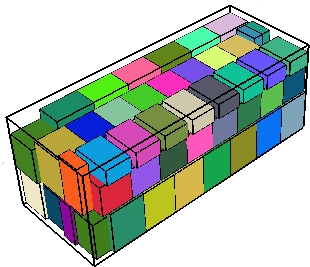
\includegraphics[scale=0.5]{img/empacotamento.jpg}
\end{figure}
\end{frame}%-------------------------------------------------------------------


\begin{frame}%-----------------------------------------------------------------
\frametitle{Atribuições de Freqüências em Telefonia de Celular}
\begin{figure}
\centering
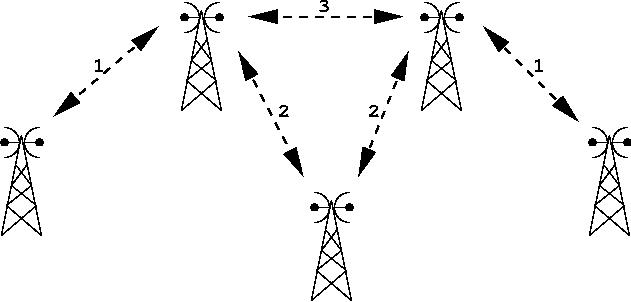
\includegraphics[scale=0.5]{img/frequencia.jpg}
\end{figure}
\end{frame}%-------------------------------------------------------------------

\subsection{Métodos de otimização}

\begin{frame}%-----------------------------------------------------------------
\frametitle{Métodos de otimização}

\begin{itemize}
\item Métodos determinísticos

\begin{itemize}
\item força-bruta
\item simplex
\item branch \& bound
\item etc.
\end{itemize}

\vspace{10pt}\item Métodos estocásticos ou probabilísticos

\begin{itemize}
\item algoritimo genético
\item colônia de formigas
\item enxame de partículas
\item simulating anneling
\item GRASP
\item evolução diferencial
\item etc.
\end{itemize}

\end{itemize}

\end{frame}%-------------------------------------------------------------------

\section{Distribuição de probabilidade}

\begin{frame}%-----------------------------------------------------------------
\frametitle{Distribuição de probabilidade}

Uma solução de um método estocástico representa uma variável aleatória pertencente a uma distribuição de probabilidade

\pause
\vspace{30pt}

\begin{block}{Distribuição de probabilidade}
Uma distribuição de probabilidade descreve a chance de uma variável assumir um valor dentre um espaço de valores possíveis
\end{block}	

\end{frame}%-------------------------------------------------------------------


\begin{frame}%-----------------------------------------------------------------
\frametitle{Exemplo}
\begin{figure}
\centering
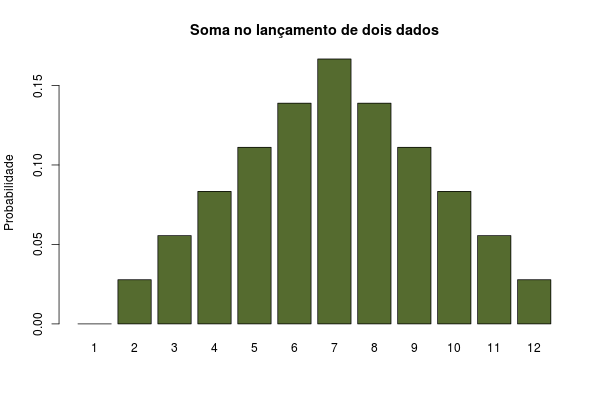
\includegraphics[scale=0.55]{img/lancamento_2_dados.png}
\end{figure}
\end{frame}%-------------------------------------------------------------------


\section{Métodos estatísticos}

\subsection{Aplicação de exemplo}

\begin{frame}%-----------------------------------------------------------------
\frametitle{Problema das P-Medianas}

\begin{block}{Descrição do problema}
Dado um grafo ponderado:
\begin{itemize}
\item escolha $p$ vértices para serem as medianas (fornecedores)
\item para vértice restante (cliente), escolha somente um mediana para atendê-lo
\item Some os pesos (distâncias) de cada vértice cliente ao seu vértice fornecedor
\item Encontre uma solução que minimize a soma dos pesos
\end{itemize}
\end{block}
\end{frame}%-------------------------------------------------------------------

\begin{frame}%-----------------------------------------------------------------
\frametitle{Problema das P-Medianas}

\begin{figure}
\centering
\includegraphics<1>[scale=1]{img/pmed1.png}
\includegraphics<2>[scale=1]{img/pmed2.png}
\end{figure}

\end{frame}%-------------------------------------------------------------------

\subsection{Comparação métodos de otimização}

\begin{frame}%-----------------------------------------------------------------
\frametitle{Modelos de otimização}

\textbf{Duas propostas para resolver esse problema:}

\begin{itemize}
\item (Método 1) Meta-heurística Multi-Start
\item (Método 2) Meta-heurística Multi-Start com um operador local aplicado sobre as soluções encontradas
\end{itemize}

\pause

\textbf{Comparação}

\begin{itemize}
\item Melhor solução encontrada em até 3 minutos de execução
\end{itemize}

\end{frame}%-------------------------------------------------------------------


\begin{frame}%-----------------------------------------------------------------
\frametitle{Modelos de otimização}

\begin{figure}
\centering
\includegraphics<1>[scale=0.5]{img/amostras}
\includegraphics<2>[scale=0.5]{img/comparao_media_amostras}
\end{figure}

\end{frame}%-------------------------------------------------------------------

\begin{frame}%-----------------------------------------------------------------
\frametitle{Modelos de otimização}

\begin{itemize}
\item Qual o número de amostras a serem utilizadas?
\item Como saber se o resultado já é conclusivo?
\end{itemize}

\end{frame}%-------------------------------------------------------------------


\section{Estatística}

\subsection{Teorema Central do Limite}

\begin{frame}%-----------------------------------------------------------------
\frametitle{Estatística}

\begin{block}{Teorema Central do Limite}
Dado um número suficientemente grande de amostras geradas de forma independente, a distribuição da média dessas amostras tende a distribuição normal.
\end{block}

\end{frame}%-------------------------------------------------------------------

\begin{frame}%-----------------------------------------------------------------
\frametitle{Estatística}

\begin{block}{Distribuição normal}
Distribuição de probabilidade paramétrica definida pelos parâmetros média ($\mu$) e desvio-padrão ($\sigma$) com a seguinte função de densidade de probabilidade:
\[
f(x, \mu, \sigma) = \dfrac{1}{2\pi\sigma^{2}}e^{-\dfrac{(x - \mu)^2}{2\sigma^2}}
\]
\end{block}

\end{frame}%-------------------------------------------------------------------

\subsection{Distribuição normal}

\begin{frame}%-----------------------------------------------------------------
\frametitle{Distribuição normal}

\begin{figure}
\centering
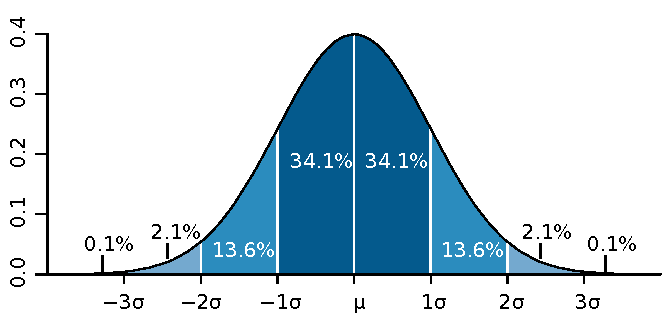
\includegraphics[scale=1]{img/Standard_deviation_diagram.pdf}
\end{figure}

\end{frame}%-------------------------------------------------------------------

\begin{frame}%-----------------------------------------------------------------
\frametitle{Distribuição normal}

\begin{figure}
\centering
\includegraphics<1>[scale=0.5]{img/densidade_media}
\end{figure}

\end{frame}%-------------------------------------------------------------------

\begin{frame}%-----------------------------------------------------------------
\frametitle{Comparação dos métodos}

\begin{figure}
\centering
\includegraphics<1>[scale=0.5]{img/densidade_n1}
\includegraphics<2>[scale=0.5]{img/densidade_n2}
\includegraphics<3>[scale=0.5]{img/densidade_n3}
\includegraphics<4>[scale=0.5]{img/densidade_n4}
\includegraphics<5>[scale=0.5]{img/densidade_n5}
\end{figure}

\end{frame}%-------------------------------------------------------------------

\subsection{Intervalo de confiança}

\begin{frame}%-----------------------------------------------------------------
\frametitle{Intervalo de Confiança}

\begin{figure}
\centering
\includegraphics<1>[scale=1]{img/ic_95}
\includegraphics<2>[scale=0.525]{img/intervalo_confianca}
\end{figure}

\end{frame}%-------------------------------------------------------------------


\section{Aplicações Web}

\begin{frame}%-----------------------------------------------------------------
\frametitle{Aplicações Web}

\begin{itemize}
\item entrada/instâncias: usuários, pageviews
\item amostras: interações geradas (cliques, tempo de sessão, download, compras, etc.)
\item objetivo: otimizar métricas relacionadas a interação do usuário

\end{itemize}

\end{frame}%-------------------------------------------------------------------

\begin{frame}%-----------------------------------------------------------------
\frametitle{KPI - Key Performance Indicator}

Exemplo de métricas:

\begin{itemize}
\item \textbf{CTR (Click-through rate)}: taxa de ocorrência de cliques

\item \textbf{RPU (revenue per user)}: receita por usuário

\item \textbf{Installations / New Users}: número de vezes que um aplicativo é instalado em um dispositivo ou browser. A métrica é utilizada como indicativo do número de novos usuários um aplicativo pode atrair dado um intervalo de tempo (dia, semana, mês, etc.)

\item \textbf{Sessions Per User}: Compara o número média de sessões um usuário gera por unidade de tempo. Exmplos: número médio de vezes que um usuário interage com um jogo, média de pesquisas feitas pelo usuário num site de buscas.

\end{itemize}
\end{frame}%-------------------------------------------------------------------



\begin{frame}%-----------------------------------------------------------------
\frametitle{Como realizar otimização em aplicações web}

\begin{itemize}
\item<1-> Cada vez que um usuário interage com a aplicação gera uma amostra única
\item<2-> Não é possível aplicar dois modelos ao mesmo usúario ao mesmo tempo.
\item<3-> Os modelos precisam ser testados ao mesmo tempo
\end{itemize}

\end{frame}%-------------------------------------------------------------------


\begin{frame}%-----------------------------------------------------------------
\frametitle{Teste A/B}

\begin{figure}
\centering
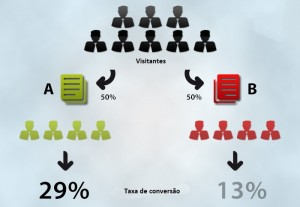
\includegraphics[scale=.8]{img/teste_ab.jpg}
\end{figure}
\end{frame}

\begin{frame}%-----------------------------------------------------------------
\frametitle{Teste A/B}

\begin{itemize}
\item Separe de forma aleatória o tráfego do site entre dois versões

\begin{itemize}
	\item \textbf{Controle:} Versão atual do site
	\item \textbf{Experimento:} Versão nova a ser testada
\end{itemize}

\vspace{10pt}\item Colete métricas de interesse (KPI's)

\vspace{10pt}\item Análise estatística dos dados coletados

\end{itemize}
\end{frame}%-------------------------------------------------------------------

\begin{frame}%-----------------------------------------------------------------
\frametitle{Casos de uso Teste A/B}

\begin{itemize}
\item Amazon
\begin{itemize}
\item Recomendações personalizadas
\item a cada 100ms de lentidão do site, o impacto negativo nas vendas chega a 100k
\end{itemize}

\item Google: cerca de 20k experimentos controlados por ano

\item Microsoft: realiza testes controlados até para encontrar erros no backend

\end{itemize}

\end{frame}%-------------------------------------------------------------------


\begin{frame}%-----------------------------------------------------------------
\frametitle{História dos experimentos aleatórios controlados}

\begin{itemize}
\item Marinha inglesa (1700)
\item Tratamento médico via sangramento (1836)
\item Higiene hospitalar (~1800)
\end{itemize}

\end{frame}%-------------------------------------------------------------------



\begin{frame}%-----------------------------------------------------------------
\frametitle{Otimização estocástica}

\begin{itemize}
\item usuários diferentes geram interações diferentes
\item um mesmo usuário gera interações diferentes ao longo do tempo
\item métricas possuem uma distribuição de probabilidade
\end{itemize}

\end{frame}%-------------------------------------------------------------------


\begin{frame}%-----------------------------------------------------------------
\frametitle{Exemplo CTR 50/50}

\begin{figure}
\centering
\includegraphics<1>[scale=0.5]{img/ab_moving_average}
\includegraphics<2>[scale=0.5]{img/ab_intervalo_confianca}
\includegraphics<3>[scale=0.5]{img/ab_gaussiana_10k}
\includegraphics<4>[scale=0.5]{img/ab_gaussiana_100k}

\end{figure}

\end{frame}%-------------------------------------------------------------------


\begin{frame}%-----------------------------------------------------------------
\frametitle{Exemplo CTR 10/90}

\begin{figure}
\centering
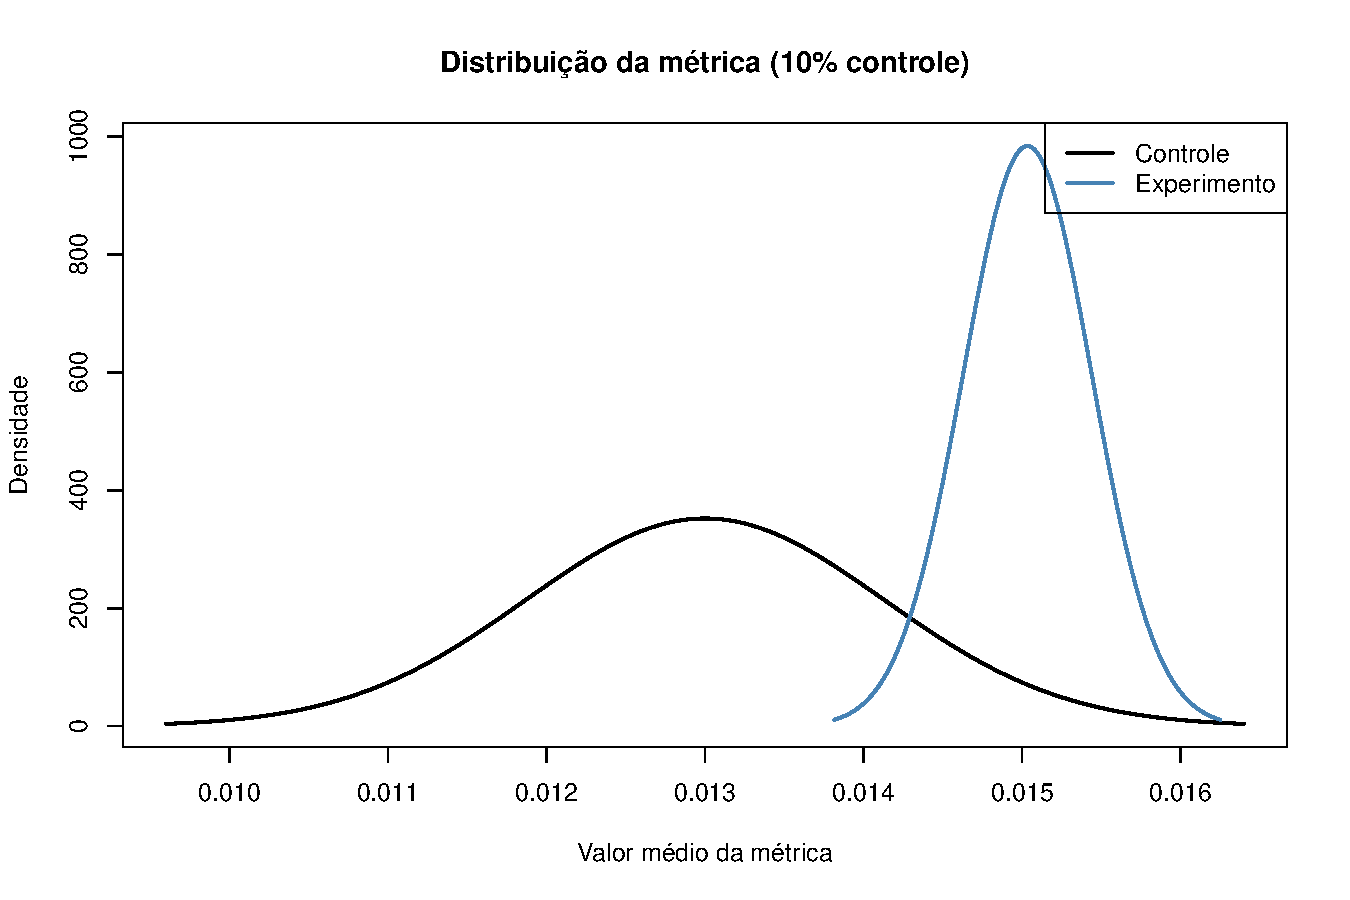
\includegraphics[scale=0.5]{img/ab_gaussiana_split10}

\end{figure}

\end{frame}%-------------------------------------------------------------------



\begin{frame}%-----------------------------------------------------------------
\frametitle{Power statistic}

\begin{figure}
\centering
\includegraphics<1>[scale=0.8]{img/power}
\includegraphics<2>[scale=0.5]{img/ab_power}
\end{figure}

\end{frame}%-------------------------------------------------------------------


\begin{frame}%-----------------------------------------------------------------
\frametitle{Outros métodos}

\begin{itemize}
\item Teste de hipótese
\item Bandit arms
\end{itemize}

\end{frame}%-------------------------------------------------------------------


\begin{frame}%-----------------------------------------------------------------
\frametitle{Melhores práticas}

\begin{itemize}
\item Defina de forma clara qual o objetivo do experimento (aumentar vendas, melhorar usabilidade, etc) e defina as métricas baseado nisso.
\item Desconsidere informação gerada por bots ( > 50\% do tráfego do Bing)
\item Comece novos experimentos com uma parte pequena do tráfego ( até 5\%)
\item Quanto mais amostras, maior a confiança dos testes
\item Não economize em teste e comece o mais rápido possível: mate as idéias ruins rapidamente e teste várias idéias para encontrar logo a que melhora a métrica em questão (cerca de 70\% dos experimentos não resultam em melhorias)

\end{itemize}

\end{frame}%-------------------------------------------------------------------


\begin{frame}%-----------------------------------------------------------------

{\LARGE\textbf{Perguntas?}}

\end{frame}%-------------------------------------------------------------------


\begin{frame}%-----------------------------------------------------------------

\begin{center}
{\LARGE\textbf{Obrigado!}}

\vspace{20pt}
Gustavo M. Zeferino \\
\url{gumaze@gmail.com}
\end{center}


\end{frame}%-------------------------------------------------------------------


%******************************************************************************
% FIM DO DOCUMENTO
%******************************************************************************
\end{document}
%******************************************************************************